\chapter{Thermochemical processes}

\section{Production of synthetic gas from a biomass}

The task is to simulate a production of synthetic gas from a biomass. One way to do it is to develop an Aspen model. The model is divided into the biomass decomposition, gasification and separation units where the solids and syngas is separated. In the simulation, the gasifier is in steady state, isothermal, and decomposition products are estimated based on the biomass ultimate analysis. Tars are not considered in the model, but ashes are taken into account as non-conventional solids. The biomass is the pine sawdust, which is a common waste product of the forest industry. The process flow diagram is presented on figure \ref{fig:Gasification}.

\begin{figure}[h!]
	\centering
	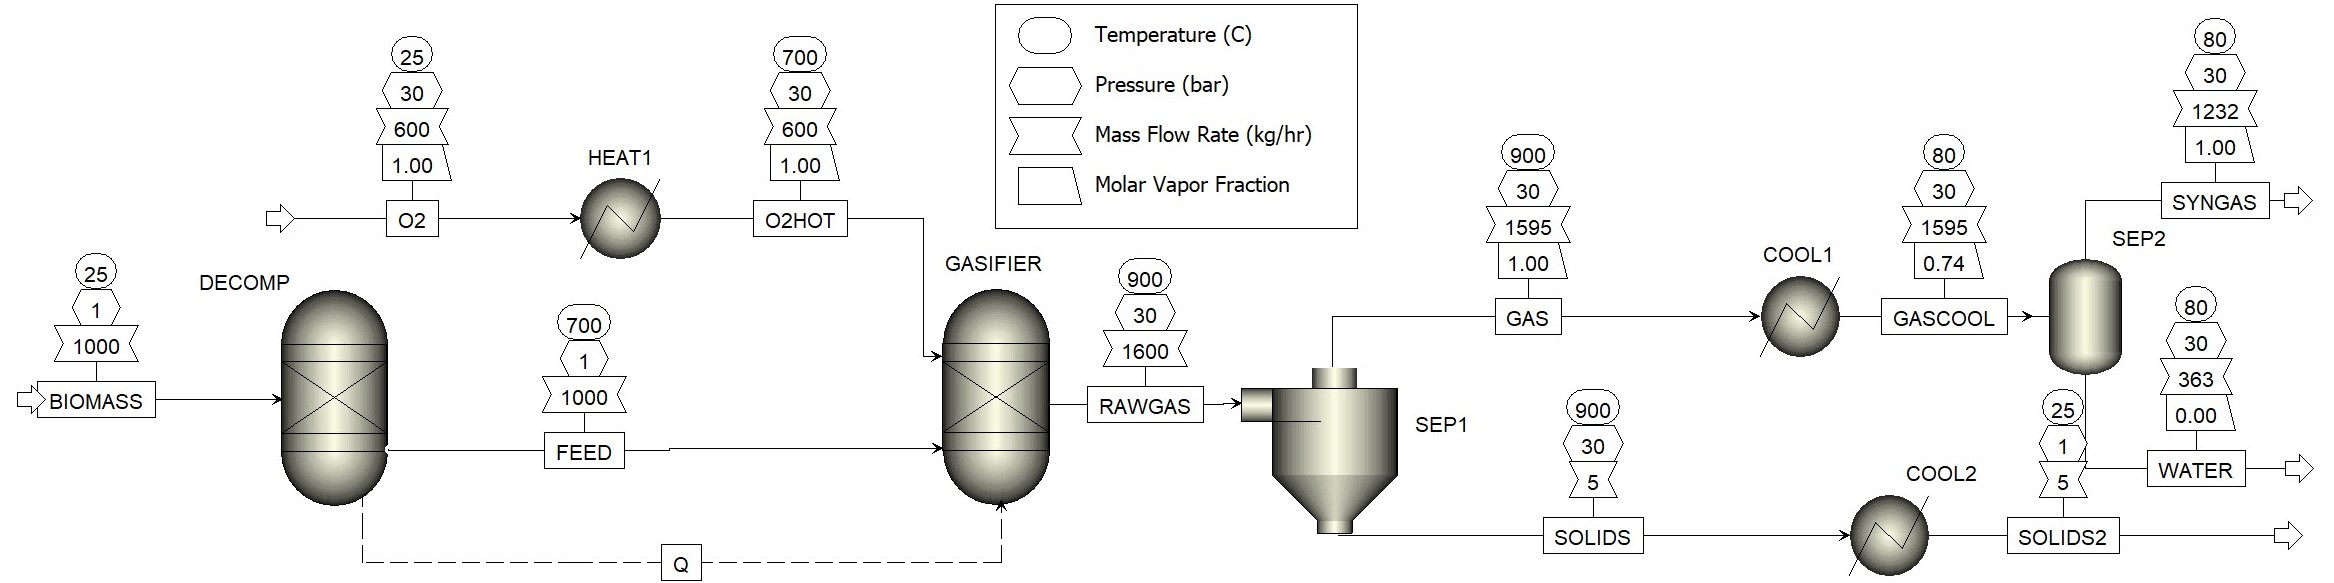
\includegraphics[width=\linewidth]{Figures/TchermochemicalProcesses/Gasification.jpeg}
	\caption{Gasification production plant}
	\label{fig:Gasification}
\end{figure}

Add all simulation's components can be found in the table \ref{tbl:Gasification_Components}.

\begin{table}[h!]
	\centering
	{\small{
	\begin{tabular}{ l|l|l|l } 
		\hline
		Component ID&	Type			&	Coponent name	&	Alias\\
		\hline 													
		BIOMASS		&	Nonconventional	&					&		\\		
		ASH			&	Nonconventional	&					&		\\
		H2			&	Conventional	&	HYDROGEN		&	H2	\\
		O2			&	Conventional	&	OXYGEN			&	O2	\\
		N2			&	Conventional	&	NITROGEN		&	N2	\\
		CO			&	Conventional	&	CARBON-MONOXIDE	&	CO	\\
		CO2			&	Conventional	&	CARBON-DIOXIDE	&	CO2	\\
		METHA-01	&	Conventional	&	METHANE			&	CH4	\\
		CARBOGRA	&	Solid			&	CARBON-GRAPHITE	&	C	\\
		S			&	Conventional	&	SULFUR			&	S 	\\
		H2S			&	Conventional	&	HYDROGEN-SULFIDE&	H2S	\\
		H3N			&	Conventional	&	AMMONIA			&	H3N \\
		\hline
	\end{tabular}}}
	\caption{Simulation component}
	\label{tbl:Gasification_Components}
\end{table}

%\subsection{Thermodynamic model} \label{CH:GasifierThermodynamics}
The next step is to select a thermodynamic model. The chosen property method is the Redlich-Kwong-Soave cubic equation of state with Boston-Mathias alpha function ($RKS-BM$). This method is suitable for non-polar or slightly polar mixtures like hydrocarbons and light gases. The data base of Aspen contains only conventional components, which means that the properties of the biomass and the coal needs to be specified manually. In the software the properties of the non-conventional components can be specified in "Method/NC Props" tab. The biomass and the ash properties can be estimated by HCOALGEN and DCOALIGT models. HCOALGEN and DCOALIGT models are used to calculate the enthalpy and density of non-conventional components, respectively. The HCOALGEN model requires these three component attributes for non-conventional components: proximate analysis results (denoted as PROXANAL in Aspen Plus), ultimate analysis results (denoted as ULTANAL in Aspen Plus), and sulfur analysis results (denoted as SULFANAL in Aspen Plus). The proximate analysis gives the weight content of moisture, fixed carbon, volatile matter and ash. The ultimate analysis gives the weight composition of coal in terms of ash, carbon, hydrogen, nitrogen, chlorine, sulfur, and oxygen. The sulfur analysis divides the sulfur content into three types, pyritic, sulfate, and organic sulfur. The DCOALIGT model requires only the two component attributes ULTANAL and SULFANAL. In Aspen Plus it is multiple correlations have been predefined to calculate the enthalpy. The HCOALGEN option codes are shown in table \ref{tbl:HCOALGEN}. 

\begin{table}[h!]
	\centering
	\resizebox{\textwidth}{!}{\begin{tabular}{clll}
		\hline
		Option Code	Value	&	Calculation	Method Parameter	&	Names Component	& 	Attributes	\\ \hline 
		\multicolumn{1}{c}{1 - Heat of Combustion}&\\
		\cline{1-1}
		1 & Boie correlation 				& 	BOIEC	& ULTANAL/SULFANAL/PROXANAL \\
		2 &	Dulong correlation				& 	DLNGC	& ULTANAL/SULFANAL/PROXANAL \\
		3 &	Grummel and	Davis correlation	&	GMLDC	& ULTANAL/SULFANAL/PROXANAL \\
		4 & Mott and Spooner correlation	& 	MTSPC	& ULTANAL/SULFANAL/PROXANAL \\
		5 & IGT correlation 				&	CIGTC	& ULTANAL/PROXANAL 			\\
		6 &	User input value 				&	HCOMB 	& ULTANAL/PROXANAL 			\\ \hline
		\multicolumn{1}{c}{2 - Standard Heat of Formation}&							\\
		\cline{1-1}
		1 &	Heat-of-combusion based correlation	&	- 	& ULTANAL/SULFANAL 			\\ 
		2 & Direct correlation 				& 	HFC		& ULTANAL/SULFANAL/PROXANAL \\ \hline
		\multicolumn{1}{c}{3 - Heat Capacity}&\\
		\cline{1-1}
		1 & Kirov correlation 				& 	CP1C 	& PROXANAL					\\
		2 & Cubic temperature equation 		& 	CP2C 	& - 						\\	\hline		
		\multicolumn{1}{c}{4 - Enthalpy Basis}&\\
		\cline{1-1}
		1 & Elements at 298.15K and 1 atm	& - & - \\
		2 & Component at 298.15 K	& - & - \\
		\cline{1-1}
		\hline
	\end{tabular}}
	\caption{HCOALGEN Option Codes}
	\label{tbl:HCOALGEN}
\end{table}

Default = 1 for each option code. In the exercise, the HCOALGEN codes for the ash are $[1~1~1~1]$, which means default values. In case of biomass the codes $[6~1~1~1]$, which means that the heat of combustion will be specified. The heat of combustion can be introduced by implementing a new non-conventional parameter in section "Pure Components". Choose the biomass from the list and select HCMOB option to introduce value $18.4 [MJ/kg]$.

As there is multiple parameters which needs to evaluated, select option "Estimate all missing parameters" from "Estimation" tab. 

%\subsection{Simulation}

Each simulation start from defining an inlet streams. Specify the biomass feed to be $1000 [kg/h]$ at $25 ^\circ C]$ and $1 [bar]$. Enter its Component attribute given in table \ref{tbl:Gasification_Components}. Add proximate, ultimate and sulphur analysis data of biomass feed in NC Solid.

\begin{table}[h!]
	\centering
	\begin{tabular}{cll}
			\hline
			Group				&	Components				&	w-\% 	\\ \hline 
			Moisture content	&	$H_2O$					&	8		\\ \hline
			\multicolumn{1}{c}{Proximate analysis}&\\
			\cline{1-1}
								&	Volatile matter (VM)	& 	82.29	\\
								& 	Fixed carbon (FC) 		& 	17.16  	\\
								&	Ash 					& 	0.55	\\ \hline
			\multicolumn{1}{c}{Ultimate  analysis}&\\
			\cline{1-1}
								& 	C 						&	50.54	\\
								&	H 						& 	7.08	\\
								&	O 						& 	41.11 	\\
								&	N 						& 	0.15	\\
								&	S 						& 	0.57	\\
								&	Ash 					&	0.55	\\ \hline
			\multicolumn{1}{c}{Sulfur  analysis}&\\
			\cline{1-1}
								&		Pyritic 			& 0			\\
								&		Sulfate 			& 0.057		\\
								&		Organic 			& 0.513		\\
			\hline
	\end{tabular}
	\caption{Characteristics of Biomass (pine sawdust)}
	\label{tbl:Biomass_Composition}
\end{table}

The biomass is defined as a non-conventional solid in Aspen Plus, as well as the ash present in the biomass. The presence of non-conventional components in the simulation need the stream class MIXINC, which is for models where both conventional solids (carbon) and non-conventional solids are present and when particle size distribution is unknown (go to Simulation-> set up-> specification-> Global setting stream class). 

When the simulation parameters are defined, the operational blocks can be introduced. The first operational unit is the decomposer. The solid biomass is decomposed at into gaseous products, which can follow further processing. For the decomposition of biomass, the DECOMP module is Aspen $RYield$ reactor where the biomass is decompose into $H_2$, $O_2$, $N_2$, $H_2O$, $S$, $C$ and ash according to the biomass ultimate analysis data at $700 [^\circ C]$ and $1 [bar]$. The RYield decomposes the biomass into the constituents shown in table \ref{tbl:DecomposerYield}.

\begin{table}[h!]
	\centering
	\resizebox{\textwidth}{!}{\begin{tabular}{ ccccccccc } 
		\hline
		Component			&	Carbon	& 	Hydrogen	&	Oxygen	&	Nitrogen	&	Sulfur		&	Ash			&	Water	\\
		\hline 										
		Yield (in mass \%)	& 	0.464968&	0.065138	&	0.3782	&	0.00138		&	0.005244	&	0.00507		&	0.08	\\
		\hline
	\end{tabular}}
	\caption{Yields for the RYIELD reactor}
	\label{tbl:DecomposerYield}
\end{table}

\begin{wrapfigure}{RO}{0.4\textwidth}
	\begin{center}
		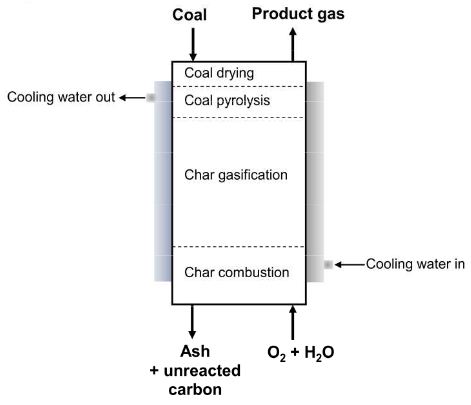
\includegraphics[width=0.4\textwidth]{Figures/TchermochemicalProcesses/Gasifier.png}
	\end{center}
	\caption{The gasifier}
	\label{fig::Gasifier}
\end{wrapfigure}  

The next operation unit to consider is the gasifier (presented on figure \ref{fig::Gasifier}). For that purpose let's use the Gibbs Reactor will simply produce an outlet in which the Gibbs free energy of the mixture is minimized. A reaction set can be attached to this reactor, but it is important to note that any parameters specified in the set will not be included in the simulation as the minimization of free energy will be the dominant simulation method. An exception to this rule is the stoichiometry of the reaction set. Without a set, stoichiometry will not be considered in the simulation; however, with an attached reaction set with stoichiometric parameters, the simulation will account for them and the outlet conditions can change. However, if a set is attached, only the components specified in the set will reach an equilibrium point; other components will be neglected. The Gibbs Reactor can be very useful if the user does not possess any data pertinent to the reaction or desires only a simulation of the equilibrium state. At the very least, the Gibbs Reactor can provide simulation estimates as a starting point for a more rigorous simulation through another reactor type.

The pressure is at $30 [bar]$ and $900 [^\circ C]$, which is a typical value for real world gasifiers. Oxygen $600 [kg/h]$ is used as the oxidizing agent, which is preheated to $700 [^\circ C]$. The possible products of the gasification were predefined to be: $H_2$, $O_2$, $N_2$, $H_2O$, $S$, $C(solid)$, $CO$, $CO_2$, $H_2S$, $CH_4$, $C$ and $NH_3$. Aspen calculated the product distributions at various conditions.

Finally, in the separation part of the simulation the solids are separated from the hot gases in SEP1, which is an Aspen SSplit. The SSPLIT assumes perfect separation of solid particles from the main stream. The SEP2 column is a flash column used to separate the condensate. For this the gases is cooled to $80 [^\circ C]$ with heat exchanger COOL1. The product of the process is the stream SYNGAS, which contains the main syngas components $CO$ and $H_2$, but also contains impurities such as $H_2S$ and $NH_3$. The product of this process need to be further purified in a separate purification facility to be useful feedstock for other processes.

The configuration of the simulation and its results are presented below:

\newpage %\subsection{Results}
\begin{figure}[h!]
	\centering
	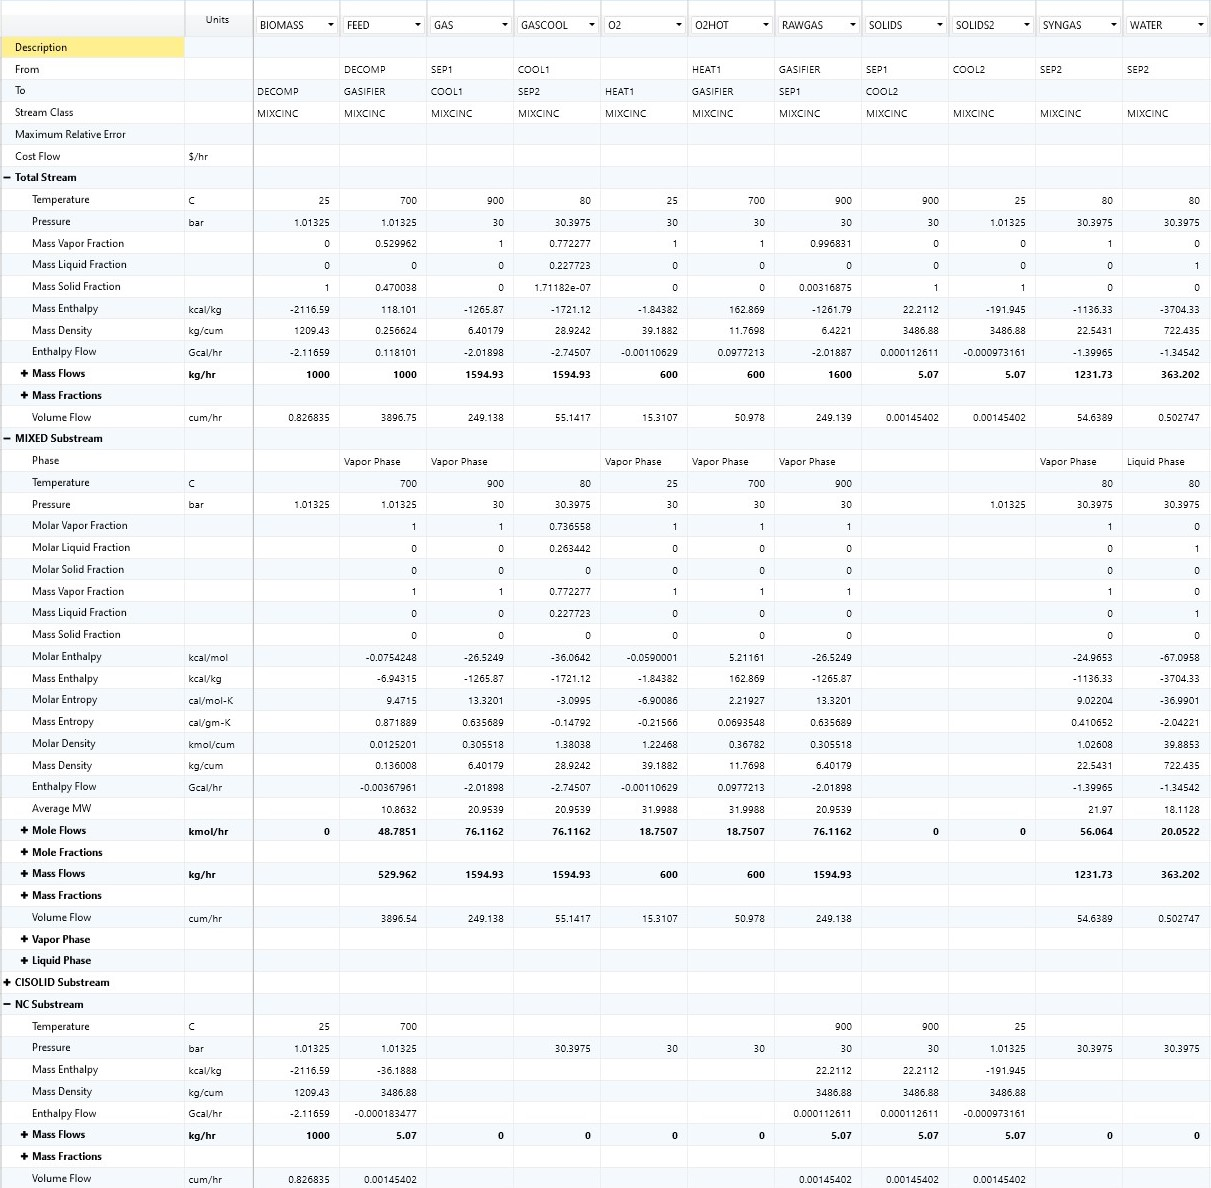
\includegraphics[width=\linewidth]{Figures/TchermochemicalProcesses/GasificationResults.jpg}
	\caption{Gasification results}
\end{figure}

\newpage
\section{The fast pyrolysis of the biomass}

Biomass fast pyrolysis is a highly non-equilibrium reaction where the main components (lignin, celluloses and hemicelluloses) are broken down into shorter molecules like acids, aldehydes, phenols, sugars and non-condensable gases. More than 200 different components have are identified
in pyrolysis oil and their share depends on the feedstock, process parameters and on the measurement equipment. Therefore, modelling of biomass fast pyrolysis is not trivial. The following assumptions will allow modelling of biomass fast pyrolysis:

\begin{itemize}
	\item Biomass, ash, char and lignin are define as non-conventional component (neither molecular weight nor molecular structure can be given); Biomass attributes are computed with AspenPlus’ built-in enthalpy and density models HCOALGEN and DCOALLIGT (for reference check chapter \ref{CH::GasifierThermodynamics})
	\item Pyrolysis is modelled with a yield reactor where user defines the pyrolysis products.
\end{itemize}

The process flow diagram is presented on figure \ref{fig:Pyrolasis}. The biomass is fed directly to the pyrolysis unit, which operates at high temperature and atmospheric pressure. Then the gaseous streams is cooled down, and two-phase mixture is separated.

\begin{figure}[h!]
	\centering
	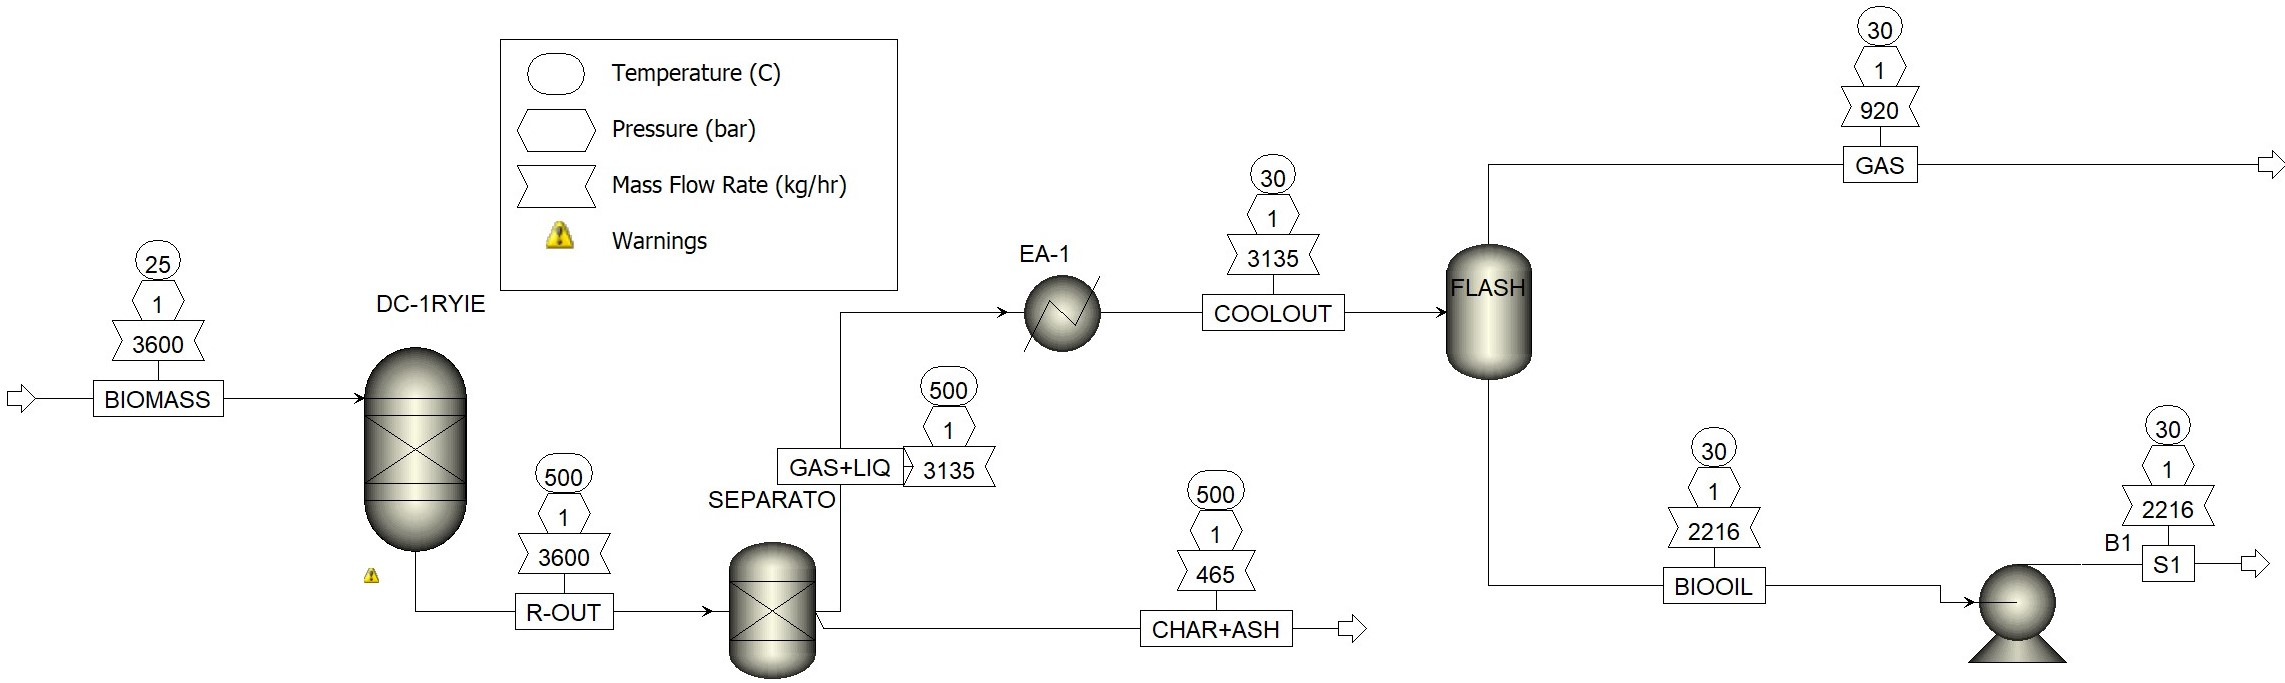
\includegraphics[width=\linewidth]{Figures/TchermochemicalProcesses/Pyrolysis.jpeg}
	\caption{Fast pyrolysis plant}
	\label{fig:Pyrolasis}
\end{figure}

%\subsection{Thermodynamic model}
Add all the conventional components in the component list as given in the table \ref{tbl:Pyrolysis_components} and non-conventional components BIOMASS, ASH, CHAR and LIGNIN. 

The thermodynamic method used in this exercise is UNIQUAC (universal quasichemical), which is an activity coefficient model used in description of phase equilibria The model is a so-called lattice model and has been derived from a first order approximation of interacting molecule surfaces in statistical thermodynamics. The model is however not fully thermodynamically consistent due to its two liquid mixture approach. In this approach the local concentration around one central molecule is assumed to be independent from the local composition around another type of molecule. The UNIQUAC model also serves as the basis of the development of the group contribution method UNIFAC, where molecules are subdivided into functional groups. In fact, UNIQUAC is equal to UNIFAC for mixtures of molecules, which are not subdivided; e.g. the binary systems water-methanol, methanol-acryonitrile and formaldehyde-DMF. 

The properties of the non-conventional components need to define. To do so by introducing default values for HCOALGEN and DCOALLIGT.

\begin{table}[h!]
	\centering
	\resizebox{\textwidth}{!}{\begin{tabular}{ccccc}
		\hline
		Group				&	Component		&	Formula			&	CAS			& Final yield [kg/kg biomass]	\\ \hline 
		\multicolumn{1}{c}{Proximate analysis}	&\\
		\cline{1-1}
							&	Carbonmonoxide 	&	$CO$			&	630-08-0	&	0,05681 \\
							&	Hydrogen 		&	$H2$ 			&	1333-74-0 	&	0,00813	\\
							&	Methane 		&	$CH_4$ 			&	74-82-8 	&	0,00048	\\
							&	Carbondioxide 	&	$CO_2$ 			&	124-38-9 	&	0,04693	\\
							&	Ethane 			&	$C_2H_6$		&	74-84-0 	&	0,00196	\\
							&	Propane 		&	$C_3H_8$		&	74-98-6 	&	0,00210	\\
							&	Ammonia 		&	$NH_3$ 			&	7664-41-7 	&	0,00172	\\
							&	Hydrogensulfide &	$H2S$			&	7783-06-4 	&	0,00075	\\	\hline 
		\multicolumn{1}{c}{Liquid / Oil}	&\\
		\cline{1-1}
							&	Phenol 			&	$C_6H_6O$ 		&	108-95-2 	&	0,04201	\\
							&	Formic Acid		& 	$CH_2O_2$ 		&	64-18-6 	&	0,1001	\\
							&	Formaldehyde 	&	$CH_2O$ 		&	50-00-0 	&	0,14865	\\
							&	Glucose 		&	$C_6H_{12}O_6$ 	&	50-99-7 	&	0,05841	\\
							&	Fluoranthene 	&	$C_{16}H_{10}$ 	&	206-44-0 	&	0,08807	\\
							&	Dihydrogenoxide &	$H_2O$ 			&	7732-18-5 	&	0,17202	\\
							&	Pyrolitic Lignin&	$NC$ 			&	$CH_{1.1}O_{0.3}$ 	&	0,14285	\\	\hline
		\multicolumn{1}{c}{Solid}	&\\
		\cline{1-1}
							&	Char 			&	NC 				&	$CH_{0.48}O_{0.23}$ &	0,12185	\\
							&	Ash 			&	NC 				&	Ash 		&	0,00716 \\ \hline
		Sum					&					&					&				&	1		\\
		\hline
	\end{tabular} }
	\caption{Characteristics of Biomass (pine sawdust)}
	\label{tbl:Pyrolysis_components}
\end{table}

%\subsection{Simulation}

In the Simulation section, Main Flowsheet, select a yield reactor and connect IN and Out streams. In the Setup sheet, set Stream class to ‘MIXNC’. This will enable calculation of non-conventional components (go to Simulation-> set up-> specification-> Global setting stream class). 

The next step is to define Biomass feed at 25 °C, 1bar and 1kg/s. Use Component Attribute given in table \ref{tbl:Biomass_Composition_Pyrolysis}. The biomass strem enters the yield reactor which represent the pyrolysis unit. The reaction works at following conditions: $1 [bar]$ and $500 [^\circ C]$. The reaction yields are shown in table \ref{tbl:Biomass_Composition_Pyrolysis}. In the reactor block, the non-conventional product components need to be defined by their analyses according to tables \ref{tbl:Lingin_Composition_Pyrolysis}, \ref{tbl:Char_Composition_Pyrolysis} and \ref{tbl:Ash_Composition_Pyrolysis}. The products compositions should be included in "Comp. Attr." tab of the reactor unit.

\begin{table}[h!]
	\centering
	\begin{subtable}[h]{0.49\textwidth}
		\resizebox{\textwidth}{!}{\begin{tabular}{cll}
			\hline
			Group						&	Components				&	w-\% 	\\ \hline 
			Moisture content			&	$H_2O$					&	10		\\ \hline
			\multicolumn{1}{c}{Proximate analysis}&\\
			\cline{1-1}
			&	Volatile matter (VM)	& 	82.73	\\
			& 	Fixed carbon (FC) 		& 	16.47  	\\
			&	Ash 					& 	0.8		\\ \hline
			\multicolumn{1}{c}{Ultimate  analysis}&\\
			\cline{1-1}
			& 	C 						&	50.64	\\
			&	H 						& 	6.18	\\
			&	O 						& 	42.22 	\\
			&	N 						& 	0.16	\\
			&	S 						& 	0.08	\\
			&	Ash 					&	0.80	\\ \hline
			\multicolumn{1}{c}{Sulfur  analysis}&\\
			\cline{1-1}
			&		Pyritic 			& 	0.0		\\
			&		Sulfate 			& 	0.0		\\
			&		Organic 			& 	0.08	\\
			\hline
		\end{tabular}}
		\caption{Biomass fuel analysis}
		\label{tbl:Biomass_Composition_Pyrolysis}
	\end{subtable}
	\hfill
	\begin{subtable}[h]{0.49\textwidth}
		\resizebox{\textwidth}{!}{\begin{tabular}{cll}
			\hline
			Group						&	Components				&	w-\% 	\\ \hline 
			Moisture content			&	$H_2O$					&	0		\\ \hline
			\multicolumn{1}{c}{Proximate analysis}&\\
			\cline{1-1}
			&	Volatile matter (VM)	& 	80.00	\\
			& 	Fixed carbon (FC) 		& 	20.00  	\\
			&	Ash 					& 	0.0		\\ \hline
			\multicolumn{1}{c}{Ultimate  analysis}&\\
			\cline{1-1}
			& 	C 						&	66.80	\\
			&	H 						& 	6.18	\\
			&	O 						& 	27.02 	\\
			&	N 						& 	0.0		\\
			&	S 						& 	0.0		\\
			&	Ash 					&	0.0		\\ \hline
			\multicolumn{1}{c}{Sulfur  analysis}&\\
			\cline{1-1}
			&		Pyritic 			& 	0.0		\\
			&		Sulfate 			& 	0.0		\\
			&		Organic 			& 	0.0 	\\
			\hline
		\end{tabular}}
		\caption{The composition of lignin}
		\label{tbl:Lingin_Composition_Pyrolysis}
	\end{subtable}
	\\	\bigskip \bigskip
	\begin{subtable}[h]{0.49\textwidth}
		\centering		
		\resizebox{\textwidth}{!}{\begin{tabular}{cll}
			\hline
			Group						&	Components				&	w-\% 	\\ \hline 
			Moisture content			&	$H_2O$					&	0		\\ \hline
			\multicolumn{1}{c}{Proximate analysis}&\\
			\cline{1-1}
			&	Volatile matter (VM)	& 	80.00	\\
			& 	Fixed carbon (FC) 		& 	20.00  	\\
			&	Ash 					& 	0.0		\\ \hline
			\multicolumn{1}{c}{Ultimate  analysis}&\\
			\cline{1-1}
			& 	C 						&	74.32	\\
			&	H 						& 	2.99	\\
			&	O 						& 	22.69 	\\
			&	N 						& 	0.0		\\
			&	S 						& 	0.0		\\
			&	Ash 					&	0.0		\\ \hline
			\multicolumn{1}{c}{Sulfur  analysis}&\\
			\cline{1-1}
			&		Pyritic 			& 	0.0		\\
			&		Sulfate 			& 	0.0		\\
			&		Organic 			& 	0.0 	\\
			\hline
		\end{tabular}}
		\caption{The composition of char}
		\label{tbl:Char_Composition_Pyrolysis}
	\end{subtable} 
	\hfill
	\begin{subtable}[h]{0.49\textwidth}
		\centering		
		\resizebox{\textwidth}{!}{\begin{tabular}{cll}
			\hline
			Group						&	Components				&	w-\% 	\\ \hline 
			Moisture content			&	$H_2O$					&	0		\\ \hline
			\multicolumn{1}{c}{Proximate analysis}&\\
			\cline{1-1}
			&	Volatile matter (VM)	& 	0.00	\\
			& 	Fixed carbon (FC) 		& 	0.00  	\\
			&	Ash 					& 	100.0	\\ \hline
			\multicolumn{1}{c}{Ultimate  analysis}&\\
			\cline{1-1}
			& 	C 						&	0.0		\\
			&	H 						& 	0.0		\\
			&	O 						& 	0.0 	\\
			&	N 						& 	0.0		\\
			&	S 						& 	0.0		\\
			&	Ash 					&	100.0	\\ \hline
			\multicolumn{1}{c}{Sulfur  analysis}&\\
			\cline{1-1}
			&		Pyritic 			& 	0.0		\\
			&		Sulfate 			& 	0.0		\\
			&		Organic 			& 	0.0 	\\
			\hline
		\end{tabular} }
		\caption{The composition of char}
		\label{tbl:Ash_Composition_Pyrolysis}
	\end{subtable}
	\caption{The composition of pyrolysis products}
\end{table}

The outlet stream from the reactor flows to the separator. The solid particles The SSPLIT assumes perfect separation of solid particles from the main stream. Then the mixture of gaseous and liquid products enter the heat exchanger, which work at $30 [^\circ C]$ and $1 [bar]$. As the results the condensation occurs. The following step is to separate vapour from the liquid phase in the flash. The flash is assumed to be adiabatic and isobaric. The liquid stream is the main product and represents the bio-oil. 

\newpage %\subsection{Results}
\begin{figure}[h!]
	\centering
	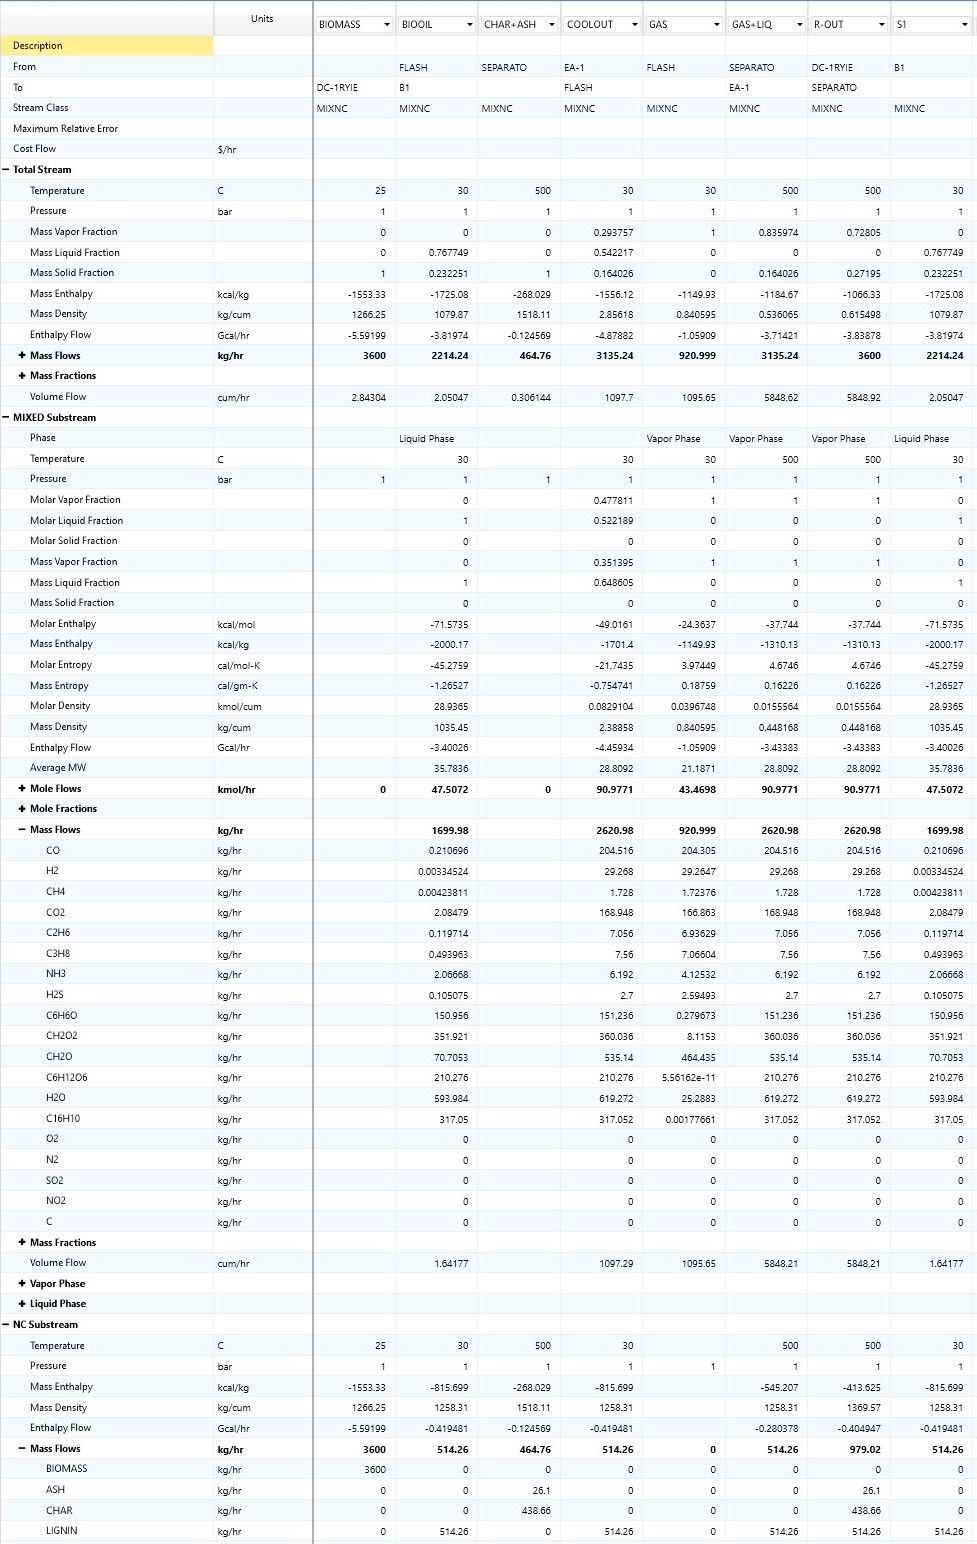
\includegraphics[width=0.91\linewidth]{Figures/TchermochemicalProcesses/PyrolysisResults.jpg}
	\caption{Fast pyrolysis results}
\end{figure}